\documentclass[11pt,a4paper]{article}

% ------------------------------------------------------------------
% Packages (all standard on Overleaf / TeX Live; compile with pdfLaTeX)
% ------------------------------------------------------------------
\usepackage[T1]{fontenc}
\usepackage[utf8]{inputenc}
\usepackage{lmodern}
\usepackage{microtype}
\usepackage[margin=2.3cm]{geometry}
\usepackage{graphicx}
\usepackage{booktabs}
\usepackage{tabularx}
\usepackage{array}
\usepackage{amsmath}
\usepackage{amssymb}      % \checkmark
\usepackage{xcolor}
\usepackage{float}
\usepackage{caption}
\usepackage{subcaption}
\usepackage{enumitem}
\usepackage{listings}
\usepackage{fancyhdr}
\usepackage{tikz}
\usetikzlibrary{arrows.meta,positioning,shapes.geometric,fit,backgrounds}
\usepackage{pgfplots}
\pgfplotsset{compat=1.17}
\usepackage[hidelinks]{hyperref}

% ------------------------------------------------------------------
% Colours and styles
% ------------------------------------------------------------------
\definecolor{brand}{HTML}{0F6B57}
\definecolor{safe}{HTML}{1F8A4C}
\definecolor{warn}{HTML}{B26A00}
\definecolor{scam}{HTML}{C2312A}
\definecolor{soft}{HTML}{EEF3F1}
\definecolor{codebg}{HTML}{F6F8F7}

\captionsetup{font=small,labelfont=bf}
\setlist{itemsep=2pt,topsep=4pt}
\setlength{\parskip}{4pt}
\renewcommand{\arraystretch}{1.25}

\lstset{
  basicstyle=\ttfamily\footnotesize,
  backgroundcolor=\color{codebg},
  frame=single, rulecolor=\color{soft},
  breaklines=true, columns=fullflexible,
  keywordstyle=\color{brand}\bfseries,
  commentstyle=\color{gray}\itshape,
  stringstyle=\color{scam!70!black},
  showstringspaces=false,
  xleftmargin=4pt, xrightmargin=4pt,
  aboveskip=8pt, belowskip=8pt
}

\setlength{\headheight}{14pt}
\pagestyle{fancy}
\fancyhf{}
\fancyhead[L]{\small Tahaffuz -- Explainable Scam Message Detector}
\fancyhead[R]{\small CT-262 Introduction to AI}
\fancyfoot[C]{\small \thepage}
\renewcommand{\headrulewidth}{0.4pt}

\newcommand{\pl}[1]{\texttt{#1}}          % Prolog / code names
\newcommand{\verdictbox}[2]{\colorbox{#1!15}{\textcolor{#1!80!black}{\textbf{#2}}}}

% ==================================================================
\begin{document}

% ------------------------------------------------------------------
% 1. Title page
% ------------------------------------------------------------------
\begin{titlepage}
  \centering
  \vspace*{1cm}
  {\large NED University of Engineering \& Technology, Karachi\par}
  \vspace{0.2cm}
  {\normalsize Department of Computer Science \& Software Engineering\par}
  \vspace{0.3cm}
  {\normalsize CT-262 \quad Introduction to Artificial Intelligence\par}
  \vspace{2.2cm}

  
\includegraphics[height=2.6cm]{figures/title_urdu.png}\par
  \vspace{0.4cm}
  {\fontsize{40}{46}\selectfont\bfseries\color{brand} Tahaffuz\par}
  \vspace{0.6cm}
  {\Large An Explainable Expert System for Detecting\\[2pt]
          Scam and Phishing Messages in Pakistan\par}
  \vspace{0.5cm}
  {\normalsize\itshape English and Roman Urdu \textbullet{} Certainty Factors (MYCIN) \textbullet{} SWI-Prolog\par}

  \vfill
  \begin{tabular}{rl}
    \textbf{Submitted by:} & Syeda Aliza Ayaz \\
    \textbf{Roll number:}  & CT-24219 \\[6pt]
    \textbf{Submitted to:} & Sir Muhammad Wasiq Noor \\
    \textbf{Course:}       & CT-262 Introduction to Artificial Intelligence \\[6pt]
    \textbf{Live Demo:}    & \url{https://huggingface.co/spaces/aliza-ayaz/Tahaffuz} \\[6pt]
    \textbf{GitHub Repo:}  & \url{https://github.com/Syeda-Aliza-Ayaz/Tahaffuz} \\[6pt]
    \textbf{Date:}         & \today
  \end{tabular}
  \vspace{1.5cm}
\end{titlepage}

% ------------------------------------------------------------------
% Abstract + contents
% ------------------------------------------------------------------
\begin{abstract}
\noindent
Fraudulent SMS and WhatsApp messages --- fake JazzCash and bank alerts, fake BISP payments,
prize draws and ``I lost my phone, send money'' requests --- are a daily problem in Pakistan,
and many of them are written in Roman Urdu. \textbf{Tahaffuz} (\emph{protection}) is a rule-based
expert system, written in SWI-Prolog, that reads a message and decides whether it is
\verdictbox{safe}{Safe}, \verdictbox{warn}{Suspicious} or \verdictbox{scam}{Scam}.
It \emph{infers} a confidence score by combining the certainty factors of the scam indicators it
finds, using the MYCIN combination formula; \emph{decides} a verdict with score bands and a gate
meta-rule; \emph{diagnoses} which kind of scam it is; and \emph{supports the user's decision} with a
recommended action and specific advice. Every verdict is explained: each indicator, the words that
triggered it, and how much it raised the score. No machine learning, training data or natural-language
processing is used. On four public SMS datasets (about 12{,}800 genuine messages) Tahaffuz rated
\textbf{no genuine message as a scam}, and on an unseen Pakistani Roman Urdu phishing dataset it
flagged \textbf{82\%} of phishing messages.
\end{abstract}

\tableofcontents
\newpage

% ------------------------------------------------------------------
% 2. Introduction
% ------------------------------------------------------------------
\section{Introduction}

\subsection{The problem}
Mobile money and SMS banking have made it easy for millions of Pakistanis to send and receive money.
They have also made it easy to steal it. A typical fraud message claims that a JazzCash or bank
account has been blocked, that the reader has won a prize on a television show, or that a
government programme such as BISP or Ehsaas has approved a payment --- and then asks for an
\emph{OTP}, a \emph{PIN}, a \emph{processing fee}, or a call to a \emph{personal mobile number}.
A study of SMS fraud in Pakistan found that most fraud messages are written in Roman Urdu
\cite{pervaiz2019}, which makes generic English spam filters a poor fit. Specifically, standard
international spam filters fail in Pakistan due to three critical gaps:
\begin{enumerate}[noitemsep]
  \item \textbf{Colloquial Roman Urdu vocabulary:} Absence of lexicons for local fraud phrases (\emph{foran bhejein}, \emph{inaam jeet liya}, \emph{khatoon/hazrat}).
  \item \textbf{Local institutional context:} Inability to distinguish legitimate 5-digit official short-codes from fraudulent 11-digit mobile phone numbers (\texttt{03xx-xxxxxxx}).
  \item \textbf{Opaque decision-making:} Black-box models provide binary classifications without explaining \emph{why} a message is dangerous or what corrective actions the victim must take.
\end{enumerate}

Two kinds of mistake matter here. Missing a scam can cost a family its savings; but wrongly flagging
a genuine bank OTP, a utility bill or a message from a relative destroys trust in the tool.
Users also need to know \emph{why} a message is dangerous, so that they learn to recognise the next one.

\subsection{Objectives}
\begin{enumerate}
  \item Detect scam and phishing messages in English and Roman Urdu, with a focus on Pakistani patterns.
  \item Use a transparent, rule-based reasoning method (certainty factors) instead of machine learning.
  \item Explain every verdict: which indicators fired, which words triggered them, and how much each contributed.
  \item Go beyond detection: diagnose the \emph{type} of scam and recommend what the user should do.
  \item Keep false positives as close to zero as possible, and measure them on real public datasets.
\end{enumerate}

\subsection{Why an expert system and not machine learning?}
\begin{itemize}
  \item \textbf{Explainability.} Every conclusion can be traced to a named rule and a matched word.
  \item \textbf{No training data needed.} Labelled Pakistani Roman Urdu fraud data is scarce; expert
        knowledge about how these scams work is not.
  \item \textbf{Zero GPU dependency and resource efficiency.} Rule inference executes in $<5$\,ms
        consuming minimal memory ($<50$\,MB), running effortlessly on low-cost edge servers without GPUs.
  \item \textbf{Regulatory compliance and auditability.} The reasoning is deterministic and inspectable by
        hand, meeting strict compliance criteria for central banks (such as State Bank of Pakistan fintech guidelines).
  \item \textbf{Easy to update.} A new scam keyword is one new fact in the knowledge base, deployed in minutes without retraining.
  \item \textbf{Defensible.} The reasoning can be checked step-by-step, which is required for this course
        and valuable for financial institutions.
\end{itemize}

\subsection{Scope}
Tahaffuz analyses the \emph{text} of SMS, WhatsApp messages and pasted emails or links, in English and
Roman Urdu. It does not read email headers, follow links, or look up phone numbers online.

% ------------------------------------------------------------------
% 3. Background
% ------------------------------------------------------------------
\section{Background}

\subsection{Expert systems}
An expert system captures the knowledge of a human expert as facts and rules, and uses an
\emph{inference engine} to apply that knowledge to a new case \cite{giarratano2005}. Its classic parts are
a \emph{knowledge base}, an \emph{inference engine}, an \emph{explanation facility} and a
\emph{user interface}. Tahaffuz has all four, plus a diagnosis and decision-support layer.

\subsection{MYCIN and certainty factors}
MYCIN was an expert system built at Stanford in the 1970s to diagnose bacterial infections and
recommend antibiotics \cite{buchanan1984}. Because medical evidence is rarely certain, each MYCIN
rule carried a \emph{certainty factor} (CF) between 0 and 1. When several rules support the same
conclusion, their CFs are combined \cite{shortliffe1975}:
\begin{equation}
  CF_{\text{combined}} = CF_1 + CF_2 \times (1 - CF_1)
  \label{eq:mycin}
\end{equation}
Each new piece of evidence closes part of the remaining gap to 1, so confidence grows but never
exceeds 1. Tahaffuz works the same way: a scam message is the ``patient'', the scam indicators are the
``symptoms'', the verdict and scam type are the ``diagnosis'', and the advice is the ``treatment''.

% ------------------------------------------------------------------
% 4. Explanation of the system
% ------------------------------------------------------------------
\section{Explanation of the System}

\subsection{Architecture}
Figure~\ref{fig:arch} shows how a message flows through Tahaffuz. Each box is a separate Prolog module.
The four stages in the middle are the core of the expert system and are described in order in
Sections~\ref{sec:inference}--\ref{sec:support}: the system first \textbf{infers} a score, then
\textbf{decides} a verdict, then \textbf{diagnoses} the scam type, and finally \textbf{supports}
the user with what to do.

\begin{figure}[H]
\centering
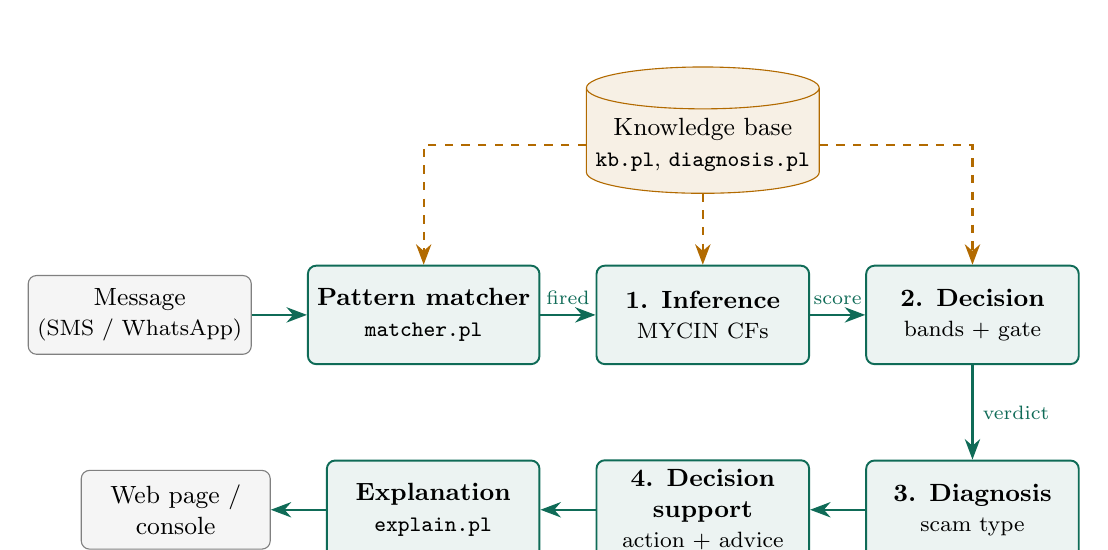
\begin{tikzpicture}[
    font=\small,
    node distance=5mm and 7mm,
    stage/.style={draw=brand, fill=brand!8, rounded corners=3pt, align=center,
                  minimum width=2.7cm, minimum height=1.25cm, line width=0.7pt},
    io/.style={draw=gray, fill=gray!8, rounded corners=3pt, align=center,
               minimum width=2.4cm, minimum height=1.0cm},
    kb/.style={draw=warn, fill=warn!10, align=center, cylinder, shape border rotate=90,
               aspect=0.18, minimum width=2.4cm, minimum height=1.2cm},
    arr/.style={-{Stealth[length=2.6mm]}, thick, brand}
  ]
  \node[io] (msg) {Message\\ \footnotesize (SMS / WhatsApp)};
  \node[stage, right=of msg] (match) {\textbf{Pattern matcher}\\ \footnotesize \pl{matcher.pl}};
  \node[stage, right=of match] (inf) {\textbf{1. Inference}\\ \footnotesize MYCIN CFs};
  \node[stage, right=of inf] (dec) {\textbf{2. Decision}\\ \footnotesize bands + gate};

  \node[stage, below=12mm of dec] (diag) {\textbf{3. Diagnosis}\\ \footnotesize scam type};
  \node[stage, left=of diag] (sup) {\textbf{4. Decision}\\ \textbf{support}\\ \footnotesize action + advice};
  \node[stage, left=of sup] (exp) {\textbf{Explanation}\\ \footnotesize \pl{explain.pl}};
  \node[io, left=of exp] (ui) {Web page /\\ console};

  \node[kb, above=9mm of inf] (kb) {Knowledge base\\ \footnotesize \pl{kb.pl}, \pl{diagnosis.pl}};

  \draw[arr] (msg) -- (match);
  \draw[arr] (match) -- node[above, font=\scriptsize]{fired} (inf);
  \draw[arr] (inf) -- node[above, font=\scriptsize]{score} (dec);
  \draw[arr] (dec) -- node[right, font=\scriptsize]{verdict} (diag);
  \draw[arr] (diag) -- (sup);
  \draw[arr] (sup) -- (exp);
  \draw[arr] (exp) -- (ui);
  \draw[arr, warn, dashed] (kb) -| (match);
  \draw[arr, warn, dashed] (kb) -- (inf);
  \draw[arr, warn, dashed] (kb) -| (dec);
\end{tikzpicture}
\caption{Architecture of Tahaffuz. Solid arrows show the flow of one message; dashed arrows show
the knowledge base being consulted.}
\label{fig:arch}
\end{figure}

\subsection{Knowledge base}
The knowledge base (\pl{src/kb.pl}) contains \emph{only facts}. The central facts are the
\textbf{indicators} (Table~\ref{tab:indicators}): each has a name, a certainty factor and the
plain-language reason shown to the user. Five of them are \textbf{action indicators}: they fire only
when the message \emph{directly asks for something of value}.

\begin{table}[H]
\centering
\small
\begin{tabularx}{\linewidth}{>{\ttfamily}l c c X}
\toprule
\textrm{\textbf{Indicator}} & \textbf{CF} & \textbf{Action} & \textbf{Fires when the message\ldots} \\
\midrule
otp\_request            & 0.85 & \checkmark & asks you to send / share an OTP or PIN \\
credential\_request     & 0.80 & \checkmark & asks for CNIC number, card number, CVV or password \\
send\_money             & 0.75 & \checkmark & asks for payment via a hidden link, to a personal number, or to unlock a prize \\
suspicious\_domain      & 0.70 & \checkmark & links to a fake or look-alike brand domain \\
personal\_number\_bait  & 0.70 & \checkmark & uses a prize, account problem or official name to make you call a personal mobile number \\
account\_blocked        & 0.70 &  & claims an account, card or SIM is blocked \\
wallet\_brand\_bait     & 0.70 &  & uses a bank / wallet name with ``verify'', ``update''\ldots \\
prize\_lottery          & 0.65 &  & mentions winning, prizes, lucky draws, \emph{inaam} \\
shortened\_link         & 0.60 &  & contains a short link (bit.ly, tinyurl\ldots) \\
threat\_penalty         & 0.55 &  & threatens legal action, fines, \emph{jurmana} \\
too\_good\_offer        & 0.45 &  & promises guaranteed profit, free gifts, \emph{muft} \\
urgency                 & 0.35 &  & ``urgent'', ``act now'', \emph{foran}, ``24 ghante'' \\
generic\_greeting       & 0.30 &  & ``dear customer'', \emph{mohtaram sarif} \\
spelling\_errors        & 0.30 &  & contains known misspellings (``acount'', ``verfy'') \\
payment\_mention        & 0.30 &  & mentions a payment (weak on its own) \\
account\_number\_request& 0.30 &  & asks for a bank account number (weak on its own) \\
raw\_link\_present      & 0.25 &  & links to an unknown website \\
\bottomrule
\end{tabularx}
\caption{The 17 indicators in the knowledge base, strongest first.}
\label{tab:indicators}
\end{table}

\noindent The knowledge base also holds the vocabulary the rules use:
\begin{itemize}
  \item \textbf{Keywords and phrases} for each indicator, in English and Roman Urdu with common spelling
        variants (e.g.\ \emph{foran / fauran / foraan}, \emph{inaam / inam}).
  \item \textbf{Request verbs} with their word order (e.g.\ \emph{send, share, bhejein, batayein}),
        \textbf{negations} (\emph{not, never, na, nahi, mat}) and \textbf{statement markers}
        (\emph{will, have, raha, diya}).
  \item \textbf{Brands and official domains} (JazzCash, Easypaisa, HBL, Meezan, BISP, NADRA, FBR,
        State Bank\ldots), \textbf{short-link hosts} and \textbf{cheap top-level domains}.
\end{itemize}
Adding knowledge is deliberately simple. For example, one line adds a new Roman Urdu urgency word:
\begin{lstlisting}[language=Prolog]
keyword(urgency, "turant").
\end{lstlisting}

\subsection{Pattern matching}
Before reasoning, the matcher (\pl{src/matcher.pl}) lower-cases the message and splits it into
sentences and words. It then checks each indicator's rule against the message. Matching is
keyword-based (no natural-language processing), but the rules are written so that common
false alarms do not fire:
\begin{itemize}
  \item Single words must match a \emph{whole word}: ``pin'' does not fire on ``shopping''.
  \item Links are found with or without \texttt{http://} (e.g.\ \texttt{bit.ly/xy12}).
  \item A request only counts when a \textbf{request verb} and a \textbf{sensitive object} appear in the
        same sentence, the verb is \textbf{not negated} and is \textbf{not a statement}.
\end{itemize}
These rules are explained further in Section~\ref{sec:language}.

% ----------------------------------------------------------------
\subsection{Inferencing}
\label{sec:inference}

\paragraph{How rules fire.}
Tahaffuz reasons in a \emph{data-driven} way, like forward chaining: the facts of the message are
given, and every indicator rule whose conditions hold \emph{fires}. A rule can depend on other
conclusions, which is where the expert knowledge lives. For example, \pl{send\_money} only fires when
a payment request is combined with a reason to distrust it:

\begin{lstlisting}[language=Prolog]
fires(send_money, Ctx, Evidence) :-
    payment_request(Ctx, Pay),          % "pay Rs 500", "500 rupay bhejein"
    payment_context(Ctx, Why),          % ... via a risky link, to a personal
    append(Pay, [Why], Evidence).       %     number, or to unlock a prize
\end{lstlisting}

\paragraph{Combining evidence.}
The CFs of all fired indicators are combined with Equation~\ref{eq:mycin}, folding from 0:

\begin{lstlisting}[language=Prolog]
combine(CF1, CF2, CF) :- CF is CF1 + CF2 * (1 - CF1).
combine_all(CFs, Score) :- foldl(combine_step, CFs, 0, Score).
\end{lstlisting}

\paragraph{Worked example.}
For the message \emph{``Your HBL debit card has been blocked. Call our helpline 0301-2345678
immediately to unblock it.''} four indicators fire (Table~\ref{tab:worked}).

\begin{table}[H]
\centering
\small
\begin{tabular}{l c l c c}
\toprule
\textbf{Indicator} & \textbf{CF} & \textbf{Matched words} & \textbf{Running score} & \textbf{Contribution} \\
\midrule
\pl{account\_blocked}      & 0.70 & blocked, card        & $0 + 0.70(1-0) = 0.700$          & +0.70 \\
\pl{wallet\_brand\_bait}   & 0.70 & hbl, unblock, card   & $0.70 + 0.70(1-0.70) = 0.910$    & +0.21 \\
\pl{personal\_number\_bait}& 0.70 & hbl, 0301-2345678    & $0.91 + 0.70(1-0.91) = 0.973$    & +0.06 \\
\pl{urgency}               & 0.35 & immediately          & $0.973 + 0.35(1-0.973) = 0.982$  & +0.01 \\
\midrule
\multicolumn{3}{l}{\textbf{Final score}} & \textbf{0.98 (98\%)} & \\
\bottomrule
\end{tabular}
\caption{Step-by-step MYCIN combination for one message.}
\label{tab:worked}
\end{table}

\paragraph{Order independence.}
Equation~\ref{eq:mycin} is commutative and associative ($1-CF$ is the product of all $(1-CF_i)$),
so the final score does \emph{not} depend on the order in which rules fire. Tahaffuz still combines
the strongest indicators first, so that the \emph{contribution} of each indicator --- how much it
raised the score --- is meaningful, and the contributions add up exactly to the final score.

% ----------------------------------------------------------------
\subsection{Decision making}
\label{sec:decision}

The inferred score is turned into a verdict in two steps (Figure~\ref{fig:decision}).

\paragraph{Step 1 --- score bands.}
\begin{center}
\small
\begin{tabular}{c c}
\toprule
\textbf{Score} & \textbf{Band} \\
\midrule
$< 0.40$ & \verdictbox{safe}{Safe} \\
$0.40 \le \text{score} < 0.70$ & \verdictbox{warn}{Suspicious} \\
$\ge 0.70$ & \verdictbox{scam}{Scam} \\
\bottomrule
\end{tabular}
\end{center}

\paragraph{Step 2 --- the gate meta-rule.}
Several signals that ask for nothing can still add up to a high score: ``Dear customer, your account
has been blocked. Act now to avoid penalty.'' scores 0.94. But a message cannot hurt you unless it \emph{asks you to do
something}. So a \textbf{Scam} verdict requires at least one \emph{action indicator}; otherwise the
verdict is capped at \textbf{Suspicious} and the user is told why. This is a rule \emph{about} the
other rules, similar to the meta-rules in MYCIN.

\begin{lstlisting}[language=Prolog]
verdict(Score, Names, Verdict) :-
    band(Score, Band),
    (   Band == scam, \+ has_action(Names)
    ->  Verdict = suspicious                 % gate: capped
    ;   Verdict = Band
    ).
\end{lstlisting}

\begin{figure}[H]
\centering
\begin{tikzpicture}[
    font=\small, node distance=6mm and 10mm,
    q/.style={draw=brand, diamond, aspect=2.2, fill=brand!6, align=center, inner sep=1pt},
    out/.style={draw, rounded corners=3pt, minimum width=2.3cm, minimum height=7mm, align=center, font=\small\bfseries},
    arr/.style={-{Stealth[length=2.4mm]}, thick}
  ]
  \node[q] (a) {score $\ge 0.70$?};
  \node[q, right=16mm of a] (b) {action\\indicator?};
  \node[out, draw=scam, fill=scam!12, text=scam!80!black, right=12mm of b] (scam) {Scam};
  \node[q, below=9mm of a] (c) {score $\ge 0.40$?};
  \node[out, draw=warn, fill=warn!12, text=warn!80!black, below=9mm of b] (sus) {Suspicious};
  \node[out, draw=safe, fill=safe!12, text=safe!80!black, below=9mm of c] (safe) {Safe};

  \draw[arr] (a) -- node[above]{yes} (b);
  \draw[arr] (b) -- node[above]{yes} (scam);
  \draw[arr] (b) -- node[right]{no (capped)} (sus);
  \draw[arr] (a) -- node[left]{no} (c);
  \draw[arr] (c) -- node[above]{yes} (sus);
  \draw[arr] (c) -- node[left]{no} (safe);
\end{tikzpicture}
\caption{Decision making: score bands followed by the gate meta-rule.}
\label{fig:decision}
\end{figure}

% ----------------------------------------------------------------
\subsection{Diagnosis}
\label{sec:diagnosis}

The verdict says \emph{how likely} a message is a scam. Diagnosis says \emph{which kind} of scam it
is --- in MYCIN terms, not just ``there is an infection'' but ``which organism''. A second rule base
(\pl{src/diagnosis.pl}) maps the indicators that fired to eight scam types (Table~\ref{tab:diagnosis}).
Several types can apply to one message; they are listed in priority order and the first is shown as
the \emph{main} diagnosis. A Safe message receives no diagnosis.

\begin{lstlisting}[language=Prolog]
diagnosis(otp_theft, F)     :- has(otp_request, F).
diagnosis(prize_fee, F)     :- has(prize_lottery, F),
                               ( has(send_money, F) ; has(personal_number_bait, F) ).
diagnosis(fake_helpline, F) :- has(personal_number_bait, F), \+ has(prize_lottery, F).
\end{lstlisting}

\begin{table}[H]
\centering
\small
\begin{tabularx}{\linewidth}{l X X}
\toprule
\textbf{Scam type (priority order)} & \textbf{Diagnosed when\ldots} & \textbf{Typical example} \\
\midrule
OTP / PIN theft               & \pl{otp\_request} fired & ``Send your OTP to verify'' \\
Personal-details theft        & \pl{credential\_request} fired & ``Confirm your CNIC and card number'' \\
Fake prize / lottery          & prize + (payment or personal number) & ``You won Rs 50,000, pay Rs 500 fee'' \\
Fake official helpline        & personal number + official name, no prize & ``HBL card blocked, call 0301\ldots'' \\
Money request                 & \pl{send\_money}, no prize & ``Ammi, send Rs 10,000 to this number'' \\
Phishing link                 & fake domain, or short link + account scare & ``Login at jazzcash-verify.xyz'' \\
Account-blocked scare         & \pl{account\_blocked} fired & ``Your account will be suspended'' \\
Too-good-to-be-true offer     & \pl{too\_good\_offer} fired & ``Earn Rs 5000 daily, 100\% guaranteed'' \\
\bottomrule
\end{tabularx}
\caption{Diagnosis rules: from fired indicators to scam types.}
\label{tab:diagnosis}
\end{table}

% ----------------------------------------------------------------
\subsection{Decision support}
\label{sec:support}

Finally, Tahaffuz helps the user decide what to do. Decision support has two parts, both reasoned
in Prolog (\pl{decision\_support/4}):

\paragraph{1. Recommended action --- a decision table on the verdict.}
\begin{center}
\small
\begin{tabularx}{0.92\linewidth}{l l X}
\toprule
\textbf{Verdict} & \textbf{Action} & \textbf{What the user is told} \\
\midrule
\verdictbox{scam}{Scam}             & block and report & Do not reply, click, call or pay. Delete the message, block the sender and report it. \\
\verdictbox{warn}{Suspicious} & verify first     & Do not act on it yet. Check with the company or person through a number or app you already trust. \\
\verdictbox{safe}{Safe}             & no action        & No scam signs found. No action needed. \\
\bottomrule
\end{tabularx}
\end{center}

\paragraph{2. Specific advice --- one or more tips for each diagnosis.}
For example, a \emph{fake official helpline} diagnosis produces: ``Official helplines use short codes
or UAN numbers, never 03xx mobile numbers. BISP only messages from 8171'' and ``Call the official
number from the card, app or website instead of the number in the message.'' If no type was
diagnosed, a general tip for the verdict is given instead, so the user always receives advice.

% ----------------------------------------------------------------
\subsection{Explanation facility}
Every result lists each fired indicator with its CF, its contribution to the score and the exact
words that triggered it. When the gate rule lowered a verdict, a note explains why. The same
explanation is available in the console:

\begin{lstlisting}
?- explain("Your HBL debit card has been blocked. Call our helpline
            0301-2345678 immediately to unblock it.").
Verdict: SCAM   (confidence 98%)
Reasons (strongest first):
  +0.70  Claims your account is blocked or suspended  [CF 0.70]
          matched: blocked, card
  +0.21  Uses a bank / mobile-wallet name to make you act  [CF 0.70]
          matched: hbl, unblock, card
  +0.06  Uses a prize, an account problem or an official name to make
         you contact a personal mobile number  [CF 0.70]
          matched: hbl, 0301-2345678
  +0.01  Creates false urgency  [CF 0.35]
          matched: immediately
Diagnosis:
  - Fake official helpline: Pretends to be a bank, wallet or government
    programme and gives a personal mobile number.
  - Account-blocked scare: Claims your account, card or SIM is blocked
    so you panic and act fast.
What to do: Do not reply, click, call or pay. Delete the message, block
            the sender and report it to your mobile operator.
  * Official helplines use short codes or UAN numbers, never 03xx ...
  * Call the official number from the card, app or website instead ...
  * Banks do not unblock accounts through SMS links or personal numbers ...
\end{lstlisting}

% ----------------------------------------------------------------
\subsection{Handling English and Roman Urdu}
\label{sec:language}
Keyword matching alone would raise many false alarms. Tahaffuz uses a few simple, explainable rules:

\begin{table}[H]
\centering
\small
\begin{tabularx}{\linewidth}{l X X}
\toprule
\textbf{Rule} & \textbf{Fires (scam)} & \textbf{Does not fire (genuine)} \\
\midrule
Negation        & ``Send your OTP now'' & ``Do \textbf{not} share your OTP'', ``OTP share \textbf{na} karein'' \\
Statement, not request & ``Please send your OTP'' & ``We \textbf{will} send you an OTP'', ``OTP bhej \textbf{raha} hoon'' \\
Word order      & ``\textbf{send} your OTP'' (English: verb, then object) & ``your OTP to confirm the transaction'' \\
                & ``OTP \textbf{bhejein}'' (Urdu: object, then verb) & \\
Ownership       & ``Send \textbf{your} account number and PIN'' & ``Should I send you \textbf{my} account number?'' \\
Specific objects& ``Share \textbf{your PIN}'' & ``Send me the location \textbf{pin}'', ``wifi password'' \\
Receipts        & ``Send Rs 500 to 0300\ldots'' & ``Transfer of Rs 500 to 0300\ldots\ was \textbf{successful}'' \\
\bottomrule
\end{tabularx}
\caption{Language rules that separate scam requests from genuine messages.}
\end{table}

\noindent The word-order rule is a neat example of linguistic knowledge in an expert system: English
is subject--verb--object, while Urdu is subject--object--verb, so the object of ``send'' is looked for
\emph{after} the verb but the object of ``bhejein'' \emph{before} it. An English verb used Urdu-style
(``OTP \textbf{send kar dein}'') is recognised by the Urdu helper word that follows it.

% ------------------------------------------------------------------
% 5. Implementation
% ------------------------------------------------------------------
\section{Implementation}

\begin{table}[H]
\centering
\small
\begin{tabularx}{\linewidth}{l X}
\toprule
\textbf{Part} & \textbf{Technology / file} \\
\midrule
Knowledge base      & SWI-Prolog facts --- \pl{src/kb.pl} (indicators, keywords, brands), \pl{src/diagnosis.pl} (scam types, advice) \\
Pattern matcher     & \pl{src/matcher.pl} --- built-in string predicates only, no external libraries \\
Inference + decision& \pl{src/inference.pl} --- MYCIN combination, bands, gate rule \\
Diagnosis + support & \pl{src/diagnosis.pl} \\
Explanation         & \pl{src/explain.pl} --- \pl{analyse/4}, \pl{assess/7}, \pl{explain/1} \\
Web layer           & \pl{server.pl} --- SWI-Prolog HTTP server; \texttt{POST /api/analyse} returns JSON \\
User interface      & \pl{web/} --- plain HTML, CSS and JavaScript; works fully offline \\
Tests               & \pl{tests/} --- 84 unit tests (plunit), 88 labelled messages, corpus evaluation \\
\bottomrule
\end{tabularx}
\caption{Implementation overview.}
\end{table}

The application can be run locally using \texttt{swipl server.pl} (or by double-clicking \texttt{start.bat}),
hosting the web interface at \texttt{http://localhost:8080}. Furthermore, to enable cross-platform and mobile
testing for evaluators and users, Tahaffuz has been deployed online to \textbf{Hugging Face Spaces}
at \url{https://huggingface.co/spaces/aliza-ayaz/Tahaffuz}. In this cloud configuration, SWI-Prolog runs
as a high-performance background daemon, communicating via HTTP JSON dispatch to serve real-time predictions
with sub-5ms response latency.

% ------------------------------------------------------------------
% 6. Evaluation
% ------------------------------------------------------------------
\section{Evaluation}

\subsection{Test data}
\begin{itemize}
  \item \textbf{Own test set} --- 88 hand-written English and Roman Urdu messages (42 scam, 46 genuine),
        including deliberately tricky genuine messages; 12 are held out and never used for tuning.
  \item \textbf{UCI SMS Spam Collection} --- 5{,}574 real English SMS \cite{uci}; used to measure false positives.
  \item \textbf{Pakistan SMS Classification} --- 4{,}895 Pakistani English SMS \cite{pksms}; used as the
        \emph{development} set: its missed fraud messages were read to improve the rules.
  \item \textbf{Roman Urdu Phishing SMS} --- 1{,}000 Pakistani SMS \cite{zenodo}; the \emph{final test}
        set, closest to the target. Never read; only summary numbers were looked at.
  \item \textbf{Mendeley SMS Phishing} --- 5{,}971 SMS, mostly Western \cite{mendeley}; a second unseen test set.
\end{itemize}
In these datasets \emph{spam} is mostly marketing, not fraud, so the useful measures are the share of
\emph{genuine} messages rated Safe, and the share of \emph{phishing} messages flagged.

\subsection{Results}

\begin{table}[H]
\centering
\small
\begin{tabular}{l r r r r}
\toprule
\textbf{Dataset} & \textbf{Genuine} & \textbf{Genuine rated} & \textbf{Phishing} & \textbf{Phishing flagged} \\
                 &                  & \textbf{Scam}          & \textbf{rated Scam}& \textbf{(Susp.\ or Scam)} \\
\midrule
Own set --- tune (36 / 40)       & 40          & 0 & 89\% & 100\% \\
Own set --- holdout (6 / 6)      & 6           & 0 & 100\% & 100\% \\
UCI (4{,}827 genuine)            & 4{,}827     & 0 & -- & -- \\
Pakistan SMS --- dev (1{,}111 fraud) & 2{,}504 & 0 & 36.1\% & 89.4\% \\
\textbf{Roman Urdu --- test} (405 phishing) & 595 & \textbf{0} & 8.9\% & \textbf{82.2\%} \\
\textbf{Mendeley --- test} (638 smishing)   & 4{,}844 & \textbf{0} & 0.0\% & 37.6\% \\
\bottomrule
\end{tabular}
\caption{Results with the rules frozen. ``Flagged'' means rated Suspicious or Scam.}
\label{tab:results}
\end{table}

\begin{figure}[H]
\centering
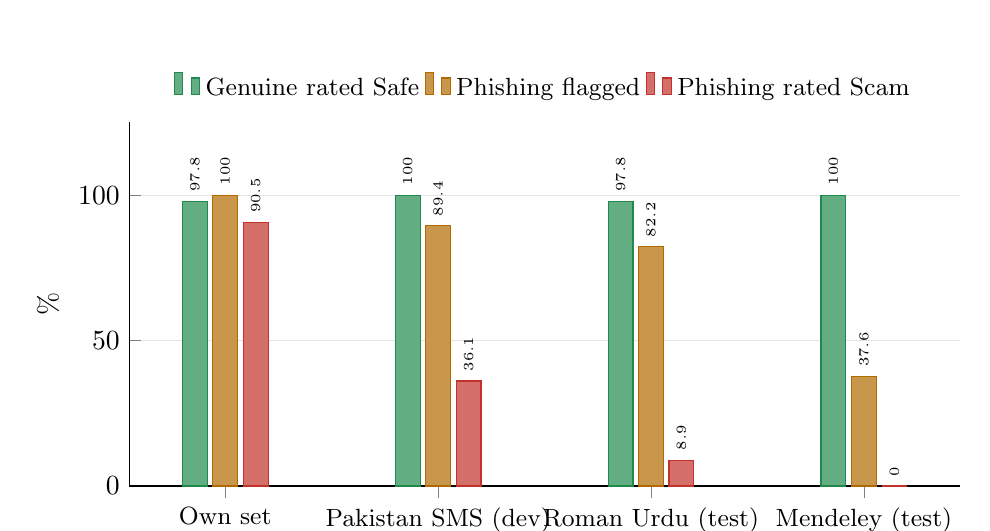
\begin{tikzpicture}
\begin{axis}[
    ybar, bar width=9pt,
    width=\linewidth, height=6.2cm,
    ymin=0,
    ylabel={\%},
    ymax=125,
    symbolic x coords={own,pk,ru,men},
    xtick=data,
    xticklabels={Own set, Pakistan SMS (dev), Roman Urdu (test), Mendeley (test)},
    xticklabel style={font=\small},
    nodes near coords, nodes near coords style={font=\tiny, rotate=90, anchor=west},
    legend style={at={(0.5,1.03)}, anchor=south, legend columns=3, font=\small, draw=none},
    enlarge x limits=0.15,
    axis lines*=left, ymajorgrids, grid style={gray!20}
  ]
  \addplot[fill=safe!70, draw=safe] coordinates
    {(own,97.8) (pk,100) (ru,97.8) (men,100)};
  \addplot[fill=warn!70, draw=warn] coordinates
    {(own,100) (pk,89.4) (ru,82.2) (men,37.6)};
  \addplot[fill=scam!70, draw=scam] coordinates
    {(own,90.5) (pk,36.1) (ru,8.9) (men,0)};
  \legend{Genuine rated Safe, Phishing flagged, Phishing rated Scam}
\end{axis}
\end{tikzpicture}
\caption{Results per dataset (own set = tune and holdout combined: 45/46 genuine Safe, 38/42 scams rated Scam).}
\label{fig:results}
\end{figure}

\subsection{Discussion}
\begin{itemize}
  \item \textbf{False positives.} Across all datasets --- roughly 12{,}800 genuine messages, slightly
        fewer distinct ones because Mendeley reuses some UCI messages --- not a single genuine message
        was rated Scam. This is the most important property for a tool people
        must trust, and it comes mainly from the gate rule and the language rules.
  \item \textbf{Cautious detection.} On the unseen Pakistani Roman Urdu test set, 82\% of phishing
        messages were flagged, but only 9\% were rated Scam. Most were rated Suspicious because the
        gate rule did not find a direct request in the form the rules expect. Tahaffuz is therefore
        \emph{precise but cautious}: when it says Scam it is almost certainly right, and it asks the
        user to verify the rest.
  \item \textbf{Generalisation.} Improvements made on the development set raised its Scam rate from
        5\% to 36\%, but did not change the Roman Urdu test results --- an honest sign that the two
        datasets phrase requests differently.
  \item \textbf{Outside Pakistan.} On Western phishing (Mendeley), only 38\% was flagged: the rules are
        written for Pakistani numbers, currencies and brands.
\end{itemize}

% ------------------------------------------------------------------
% 7. Market use case
% ------------------------------------------------------------------
\section{Market Use Case}

\subsection{Who needs it}
\begin{itemize}
  \item \textbf{Mobile Financial Services (MFS) and wallets} (JazzCash, Easypaisa, SadaPay, NayaPay), whose
        platforms are primary targets for account takeover, OTP harvesting and unauthorized fund transfers.
  \item \textbf{Commercial banks} (HBL, Meezan, UBL, Bank Alfalah), whose brands are routinely impersonated
        via fake blocked-card and helpline alerts.
  \item \textbf{Telecom operators} (Jazz, Telenor, Zong, Ufone) and state regulators (PTA), who can screen
        and block smishing broadcasts at the SMSC (Short Message Service Center) gateway.
  \item \textbf{Everyday citizens and vulnerable populations}, especially first-time smartphone users,
        elderly relatives, and BISP / Ehsaas beneficiaries who face targeted prize and welfare deception.
\end{itemize}

\subsection{How it could be deployed}
\begin{table}[H]
\centering
\small
\begin{tabularx}{\linewidth}{l X X}
\toprule
\textbf{Channel} & \textbf{How} & \textbf{Benefit} \\
\midrule
Banking / wallet app & ``Check a message'' button, calling the Tahaffuz API & Customers verify before they act; fewer fraud claims \\
WhatsApp / SMS bot   & Users forward a suspicious message and get the verdict and advice back & Reaches users who will not install a new app \\
Telecom operator     & Screen messages from unknown senders and add a warning label & Stops scams before they reach the user \\
Complaint triage     & Sort reported messages by diagnosed scam type & Investigators see which scams are trending \\
Awareness campaigns  & Show the explanation as a teaching tool & Users learn to recognise the next scam themselves \\
\bottomrule
\end{tabularx}
\caption{Possible deployments.}
\end{table}

\subsection{Why Tahaffuz fits this market}
\begin{itemize}
  \item \textbf{Explainable and auditable.} Every warning comes with clear reasons and actionable advice,
        building user trust and satisfying central bank (State Bank of Pakistan) fintech compliance rules
        better than black-box machine learning.
  \item \textbf{Local and bilingual.} Roman Urdu, Pakistani brands, BISP / Ehsaas patterns, 03xx mobile numbers
        and local rupee denominations are built into the rule base --- generic global spam filters miss these.
  \item \textbf{Zero false alarms on genuine messages.} Zero genuine messages rated Scam across approximately 12{,}800 real evaluation messages.
  \item \textbf{Ultra-lightweight execution.} Operates with sub-5ms inference latency and negligible memory ($<50$\,MB),
        requiring no GPUs and running seamlessly on edge hardware or cloud microservices.
  \item \textbf{Instant knowledge adaptation.} New scam variants (such as newly launched government schemes)
        are neutralised within minutes by declaring a single Prolog fact, eliminating dataset collection and model retraining cycles.
  \item \textbf{Complete data privacy.} Message text is evaluated on-device or within the financial institution's
        private perimeter; no user data is leaked to foreign third-party LLM APIs.
\end{itemize}

\subsection{Business model}
A free consumer version (web page or WhatsApp bot) for awareness, and a paid API for banks, wallets
and operators who integrate it into their own apps and networks, with a maintained, regularly updated
knowledge base as the main product.

% ------------------------------------------------------------------
% 8. Screenshots
% ------------------------------------------------------------------
\section{Screenshots}

\begin{figure}[H]
\centering
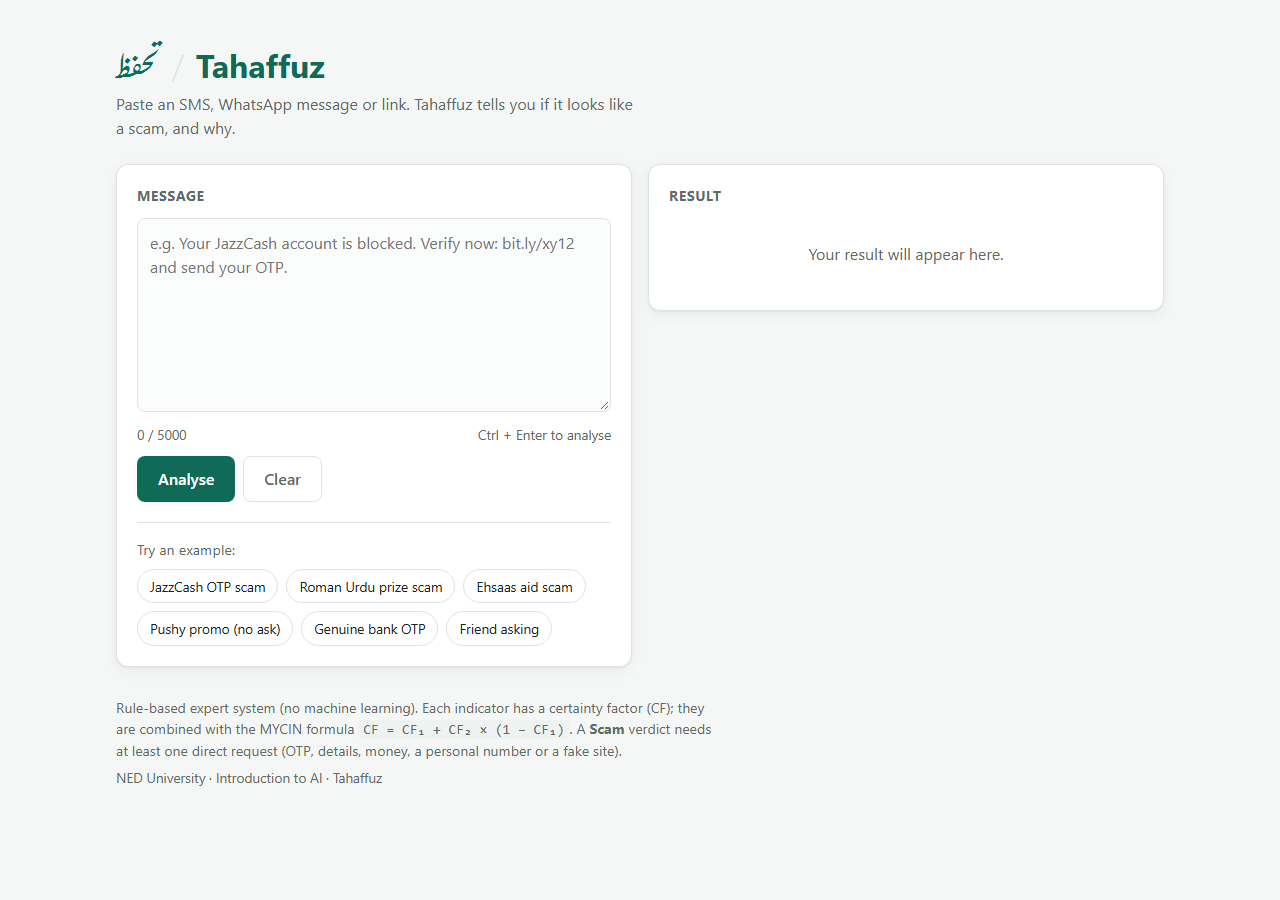
\includegraphics[width=0.92\linewidth]{figures/ss_home.png}
\caption{Home page: message box, example buttons and an empty result panel.}
\end{figure}

\begin{figure}[H]
\centering
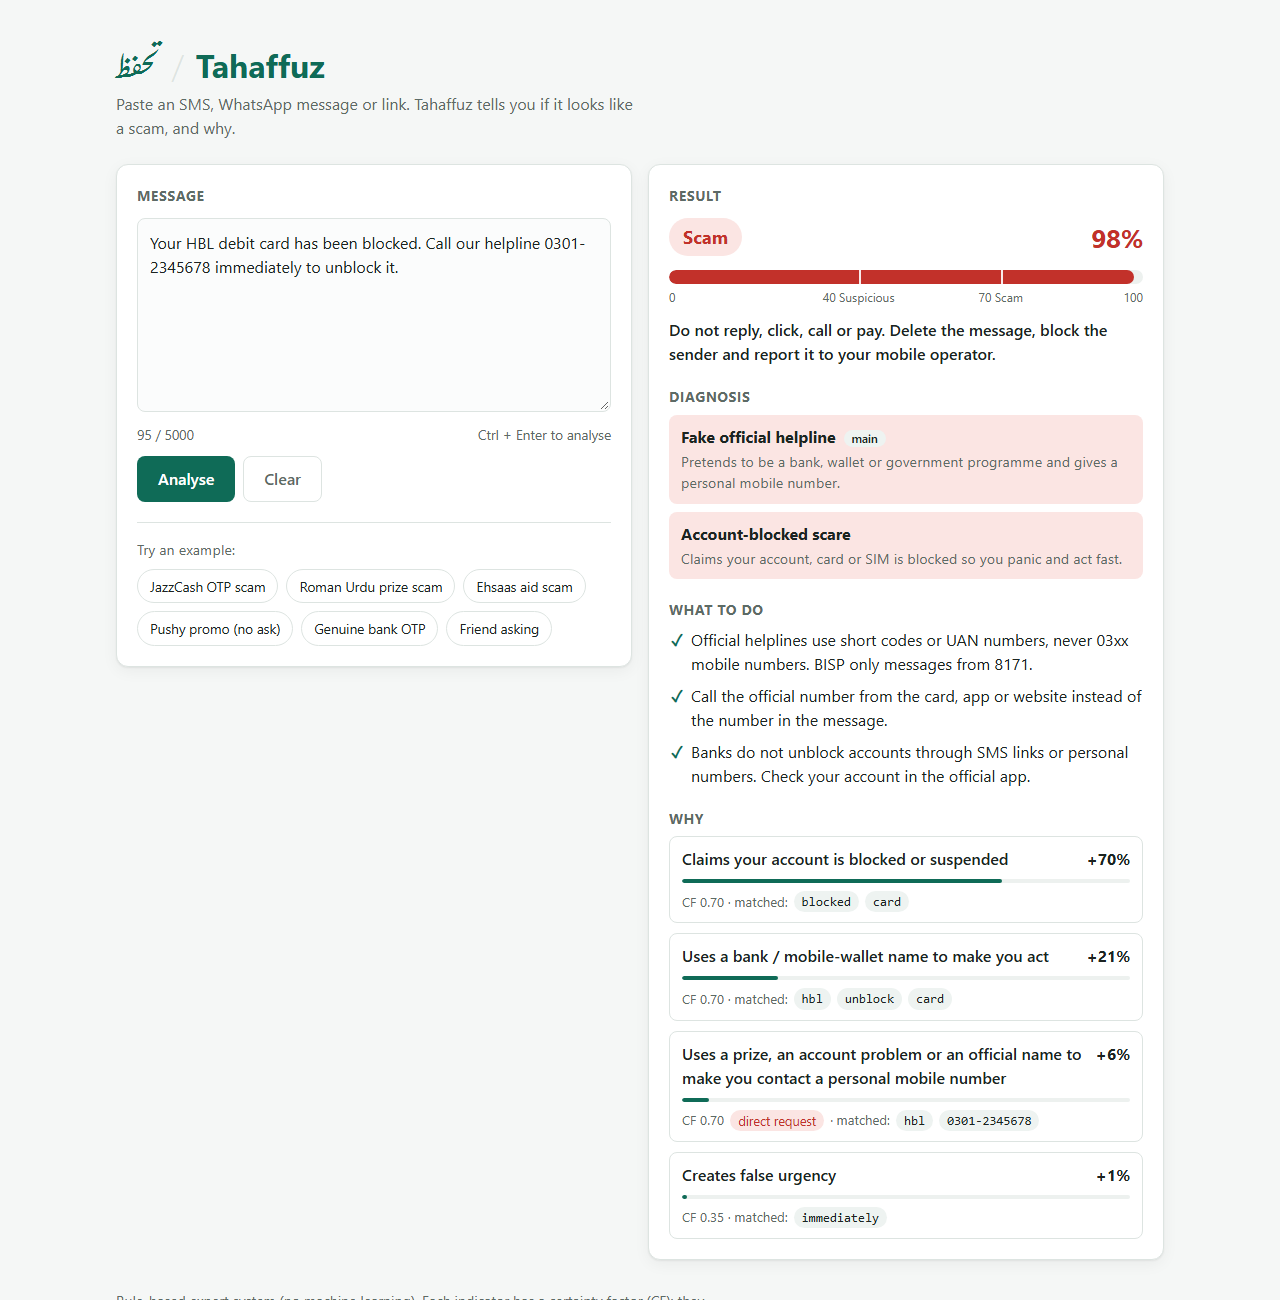
\includegraphics[width=0.92\linewidth]{figures/ss_scam.png}
\caption{\textbf{Scam} (98\%): a fake HBL helpline. The page shows the recommended action, the
diagnosis (\emph{Fake official helpline}, \emph{Account-blocked scare}), specific advice, and every
reason with its CF, contribution and matched words.}
\end{figure}

\begin{figure}[H]
\centering
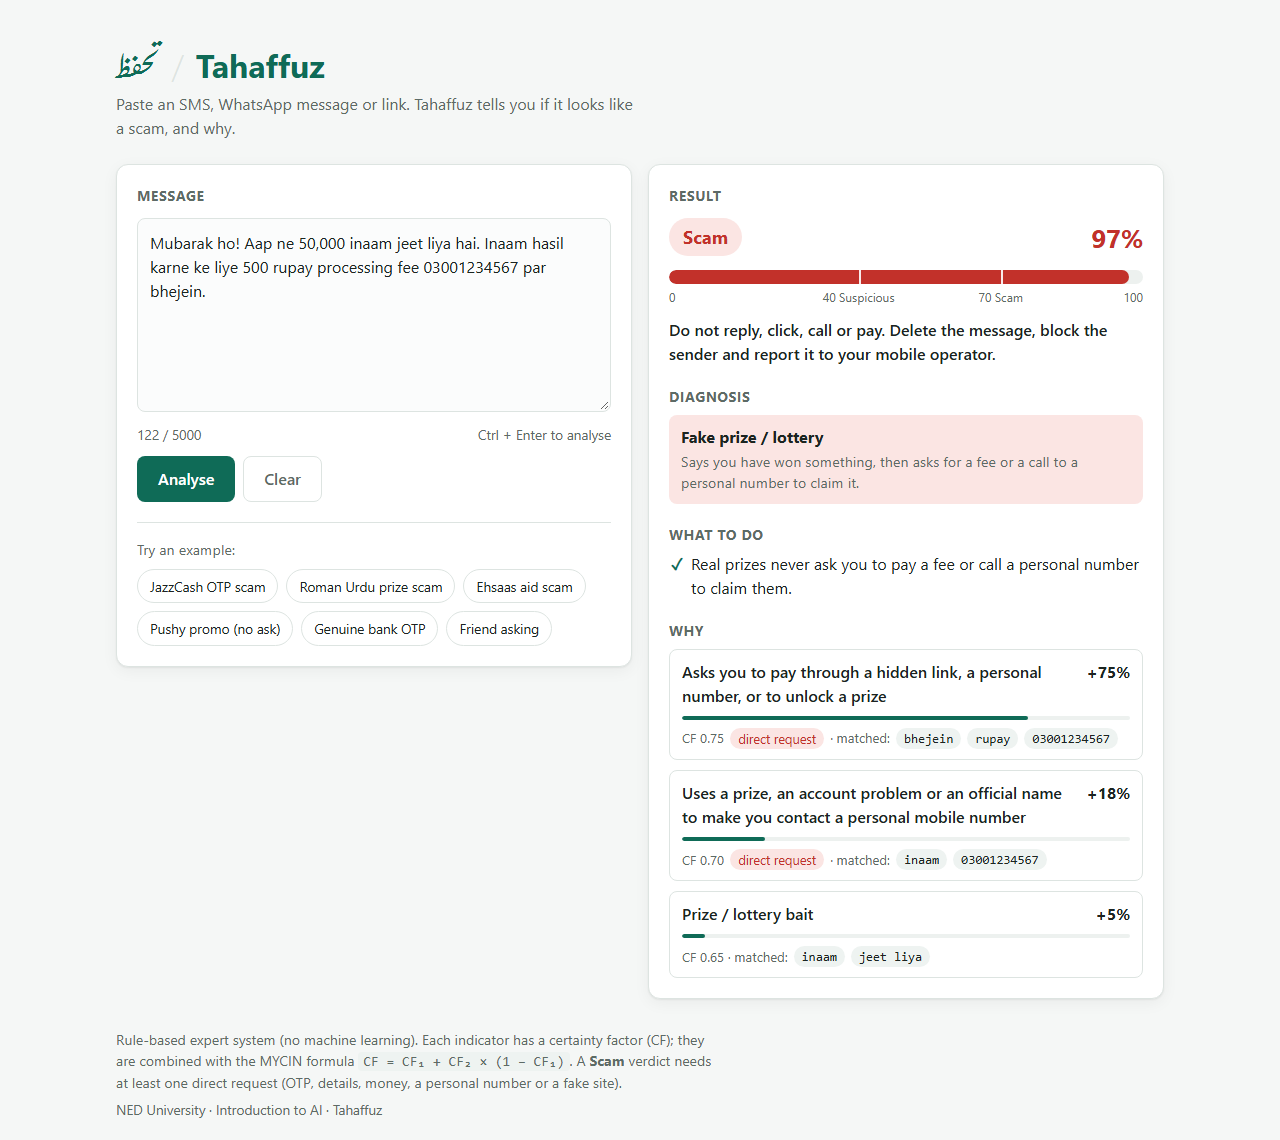
\includegraphics[width=0.92\linewidth]{figures/ss_roman.png}
\caption{\textbf{Scam} (97\%) for a Roman Urdu prize message: \emph{inaam jeet liya},
\emph{processing fee}, \emph{bhejein} and a personal number. Diagnosis: \emph{Fake prize / lottery}.}
\end{figure}

\begin{figure}[H]
\centering
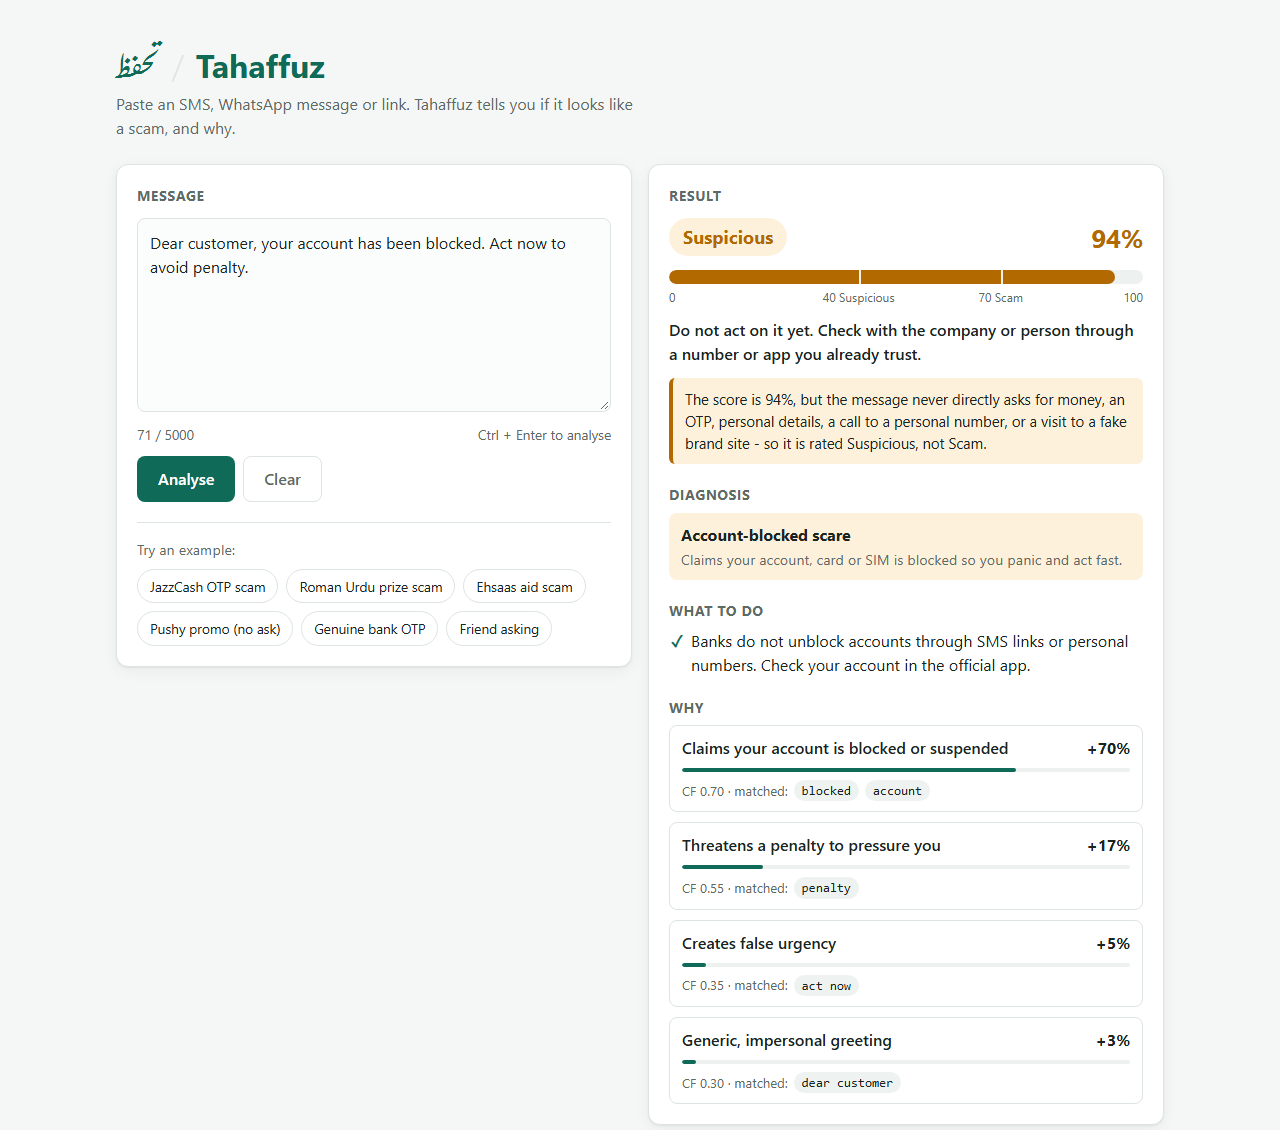
\includegraphics[width=0.92\linewidth]{figures/ss_suspicious.png}
\caption{\textbf{Suspicious} (94\%) --- the gate rule in action. Account-blocked, penalty, urgency and
greeting signals push the score into the Scam band, but nothing is directly requested, so the verdict is
capped at Suspicious and the yellow note explains why.}
\end{figure}

\begin{figure}[H]
\centering
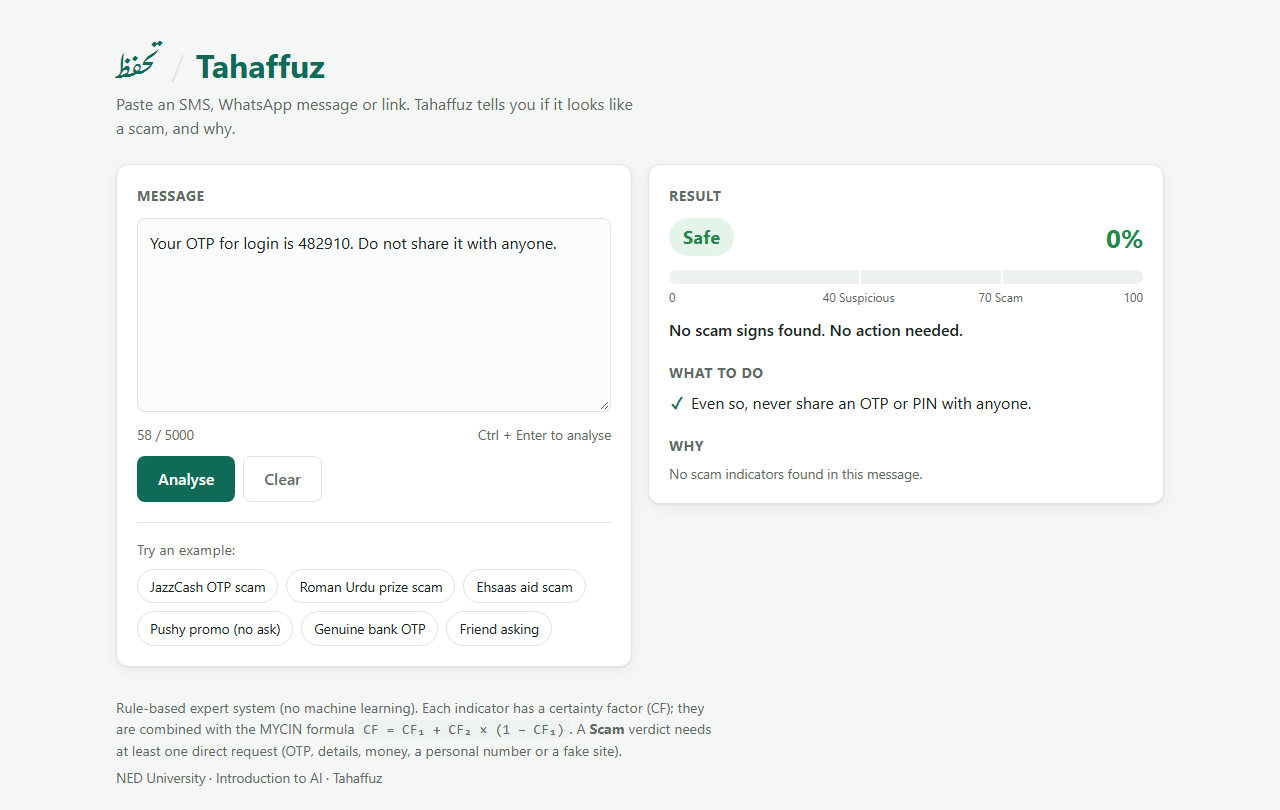
\includegraphics[width=0.92\linewidth]{figures/ss_safe.png}
\caption{\textbf{Safe} (0\%): a genuine bank OTP that says ``Do not share it with anyone''. The negation
rule stops the OTP-request indicator from firing.}
\end{figure}

% ------------------------------------------------------------------
% 9. Limitations and future work
% ------------------------------------------------------------------
\section{Limitations and Future Work}

\paragraph{Limitations.}
\begin{itemize}
  \item Keyword-based: a scam written with words the knowledge base does not contain is missed.
  \item Roman Urdu spelling varies endlessly; only the listed variants are recognised
        (e.g.\ \emph{foran} and \emph{fauran}, but not \emph{fouran}).
  \item Negation and statement detection look only at the word next to the verb, not at full grammar.
  \item Scams with no direct request (e.g.\ job offers) are rated Suspicious, not Scam, by design.
  \item The brand and official-domain lists are maintained by hand.
  \item Email headers, link destinations and phone-number reputation are not checked.
  \item The test sets have weaknesses: the own set was written by the author, the Pakistan SMS set is
        partly LLM-paraphrased, and the Roman Urdu set is probably template-generated.
\end{itemize}

\paragraph{Future work.}
\begin{itemize}
  \item Collect real, consented Pakistani scam messages to build a stronger test set.
  \item Add Urdu-script (Nastaliq) keywords and more Roman Urdu spelling variants.
  \item Host the server online: \textbf{Completed} --- deployed to Hugging Face Spaces for live public web access at \url{https://huggingface.co/spaces/aliza-ayaz/Tahaffuz}.
  \item Develop a WhatsApp bot or an Android SMS share integration calling the hosted API.
\end{itemize}

% ------------------------------------------------------------------
% 10. Conclusion
% ------------------------------------------------------------------
\section{Conclusion}
Tahaffuz shows that a classic, transparent expert system is still a strong tool for a real, local
problem. Using MYCIN-style certainty factors, it \textbf{infers} how likely a message is a scam,
\textbf{decides} a verdict with score bands and a gate meta-rule, \textbf{diagnoses} which of eight
scam types it is, and \textbf{supports} the user with a recommended action and specific advice ---
all explained in plain language. It understands Pakistani scam patterns in English and Roman Urdu,
and on about 12{,}800 real genuine messages it never raised a false Scam alarm. Its main weakness
is caution: many real scams are flagged as Suspicious rather than Scam, which future work on the
knowledge base can improve without changing the reasoning method.

% ------------------------------------------------------------------
% References
% ------------------------------------------------------------------
\begin{thebibliography}{9}
\small

\bibitem{shortliffe1975}
E.~H. Shortliffe and B.~G. Buchanan,
``A model of inexact reasoning in medicine,''
\emph{Mathematical Biosciences}, vol.~23, no.~3--4, pp.~351--379, 1975.

\bibitem{buchanan1984}
B.~G. Buchanan and E.~H. Shortliffe (eds.),
\emph{Rule-Based Expert Systems: The MYCIN Experiments of the Stanford Heuristic Programming Project}.
Addison-Wesley, 1984.

\bibitem{giarratano2005}
J.~C. Giarratano and G.~D. Riley,
\emph{Expert Systems: Principles and Programming}, 4th~ed. Thomson Course Technology, 2005.

\bibitem{russell2020}
S.~Russell and P.~Norvig,
\emph{Artificial Intelligence: A Modern Approach}, 4th~ed. Pearson, 2020.

\bibitem{swipl}
J.~Wielemaker, T.~Schrijvers, M.~Triska and T.~Lager,
``SWI-Prolog,'' \emph{Theory and Practice of Logic Programming}, vol.~12, no.~1--2, pp.~67--96, 2012.

\bibitem{pervaiz2019}
F.~Pervaiz \emph{et al.},
``An assessment of SMS fraud in Pakistan,''
in \emph{Proc.\ ACM SIGCAS Conference on Computing and Sustainable Societies (COMPASS)}, 2019.

\bibitem{uci}
T.~A. Almeida and J.~M. G\'omez Hidalgo,
``SMS Spam Collection,'' UCI Machine Learning Repository. CC BY 4.0.

\bibitem{mendeley}
S.~Mishra and D.~Soni,
``SMS Phishing Dataset for Machine Learning and Pattern Recognition,''
Mendeley Data, v1, 2022. doi:10.17632/f45bkkt8pr.1. CC BY 4.0.

\bibitem{zenodo}
G.~Siddiq,
``Roman Urdu Phishing SMS Dataset for Smishing Detection Research,''
Zenodo, v1.0.0, 2026. doi:10.5281/zenodo.21810885. CC BY 4.0.

\bibitem{pksms}
``Pakistan SMS Classification Dataset,'' Kaggle (muhammadhumyun), via GitHub
\texttt{usamabhatti1998/pakistan\_sms\_classification}.

\end{thebibliography}

\end{document}
